\documentclass{vkr}
\usepackage[english, russian]{babel} % переносы
\usepackage{graphicx} % для вставки картинок
\graphicspath{{images/}} % путь к изображениям
\usepackage[hidelinks]{hyperref}
\usepackage{float} % определяет метод H для рисунка с переносом на следующую страницу, ели не помещается
\usepackage{pdflscape}
\addto{\captionsrussian}{\renewcommand{\refname}{СПИСОК ИСПОЛЬЗОВАННЫХ ИСТОЧНИКОВ}}
\usepackage{xltabular} % для вставки таблиц
\usepackage{makecell}
\renewcommand\theadfont{} % шрифт в /thead
\usepackage{array} % для определения новых типов столбцов таблиц
\newcolumntype{T}{>{\centering\arraybackslash}X} % новый тип столбца T - автоматическая ширина столбца с выравниванием по центру
\newcolumntype{R}{>{\raggedleft\arraybackslash}X} % новый тип столбца R - автоматическая ширина столбца с выравниванием по правому краю
\newcolumntype{C}[1]{>{\centering\let\newline\\\arraybackslash\hspace{0pt}}m{#1}} % новый тип столбца C - фиксированная ширина столбца с выравниванием по центру
\newcolumntype{r}[1]{>{\raggedleft\arraybackslash}p{#1}} % новый тип столбца r - фиксированная ширина столбца с выравниванием по правому краю
\newcommand{\centrow}{\centering\arraybackslash} % командой \centrow можно центрировать одну ячейку (заголовок) в столбце типа X или p, оставив в оcтальных ячейках другой тип выравнивания
\newcommand{\finishhead}{\endhead\hline\endlastfoot}
\newcommand{\continuecaption}[1]{\captionsetup{labelformat=empty} \caption[]{#1}\\ \hline }
\usepackage{etoolbox}
\AtBeginEnvironment{xltabular}{\refstepcounter{tablecnt}} % подсчет таблиц xltabular, обычные таблицы подсчитываются в классе

\usepackage[tableposition=top]{caption} % подпись таблицы вверху
\captionsetup{strut=off}
\setlength{\intextsep}{0pt} % Vertical space above & below [h] floats
\setlength{\textfloatsep}{0pt} % Vertical space below (above) [t] ([b]) floats
\DeclareCaptionLabelFormat{gostfigure}{Рисунок #2} %подпись рисунка
\DeclareCaptionLabelFormat{gosttable}{Таблица #2} %подпись таблицы
\DeclareCaptionLabelSeparator{gost}{~--~} %разделитель в рисунках и таблицах
\captionsetup{labelsep=gost}
\captionsetup[figure]{aboveskip=10pt,belowskip=4mm,justification=centering,labelformat=gostfigure} % настройка подписи рисунка
\captionsetup[table]{font={stretch=1.41},skip=0pt,belowskip=0pt,aboveskip=8.5pt,singlelinecheck=off,labelformat=gosttable} % настройка подписи таблицы

\setlength{\LTpre}{8mm} % отступ сверху таблицы
\setlength{\LTpost}{6mm} % отступ снизу таблицы

\usepackage{enumitem}
\setlist{nolistsep,wide=\parindent,itemindent=*} % отступы вокруг списков, выравнивание с учетом разделителя

\usepackage{color} %% это для отображения цвета в коде
\usepackage{listings} %% листинги кода
\setmonofont[Scale=0.7]{Verdana} % моноширный шрифт для листинга

\definecolor{codegreen}{rgb}{0,0.6,0}
\definecolor{codegray}{rgb}{0.5,0.5,0.5}
\definecolor{codepurple}{rgb}{0.58,0,0.82}

\lstset{ %
language=C,                 % выбор языка для подсветки (здесь это С)
numbers=left,               % где поставить нумерацию строк (слева\справа)
numberstyle=\tiny,           % размер шрифта для номеров строк
stepnumber=1,                   % размер шага между двумя номерами строк
numbersep=5pt,                % как далеко отстоят номера строк от подсвечиваемого кода
commentstyle=\color{codegreen},
keywordstyle=\color{magenta},
numberstyle=\tiny\color{codegray},
stringstyle=\color{codepurple},
basicstyle=\linespread{0.95}\ttfamily,
backgroundcolor=\color{white}, % цвет фона подсветки - используем \usepackage{color}
showspaces=false,            % показывать или нет пробелы специальными отступами
showstringspaces=false,      % показывать или нет пробелы в строках
showtabs=false,             % показывать или нет табуляцию в строках
frame=single,              % рисовать рамку вокруг кода
tabsize=2,                 % размер табуляции по умолчанию равен 2 пробелам
captionpos=t,              % позиция заголовка вверху [t] или внизу [b] 
breaklines=true,           % автоматически переносить строки (да\нет)
breakatwhitespace=false, % переносить строки только если есть пробел
escapeinside={\%*}{*)}   % если нужно добавить комментарии в коде
}

\makeatletter % чтобы допускались русские комментарии в листингах
\lst@InputCatcodes
\def\lst@DefEC{%
 \lst@CCECUse \lst@ProcessLetter
  ^^80^^81^^82^^83^^84^^85^^86^^87^^88^^89^^8a^^8b^^8c^^8d^^8e^^8f%
  ^^90^^91^^92^^93^^94^^95^^96^^97^^98^^99^^9a^^9b^^9c^^9d^^9e^^9f%
  ^^a0^^a1^^a2^^a3^^a4^^a5^^a6^^a7^^a8^^a9^^aa^^ab^^ac^^ad^^ae^^af%
  ^^b0^^b1^^b2^^b3^^b4^^b5^^b6^^b7^^b8^^b9^^ba^^bb^^bc^^bd^^be^^bf%
  ^^c0^^c1^^c2^^c3^^c4^^c5^^c6^^c7^^c8^^c9^^ca^^cb^^cc^^cd^^ce^^cf%
  ^^d0^^d1^^d2^^d3^^d4^^d5^^d6^^d7^^d8^^d9^^da^^db^^dc^^dd^^de^^df%
  ^^e0^^e1^^e2^^e3^^e4^^e5^^e6^^e7^^e8^^e9^^ea^^eb^^ec^^ed^^ee^^ef%
  ^^f0^^f1^^f2^^f3^^f4^^f5^^f6^^f7^^f8^^f9^^fa^^fb^^fc^^fd^^fe^^ff%
  ^^^^20ac^^^^0153^^^^0152%
  % Basic Cyrillic alphabet coverage
  ^^^^0410^^^^0411^^^^0412^^^^0413^^^^0414^^^^0415^^^^0416^^^^0417%
  ^^^^0418^^^^0419^^^^041a^^^^041b^^^^041c^^^^041d^^^^041e^^^^041f%
  ^^^^0420^^^^0421^^^^0422^^^^0423^^^^0424^^^^0425^^^^0426^^^^0427%
  ^^^^0428^^^^0429^^^^042a^^^^042b^^^^042c^^^^042d^^^^042e^^^^042f%
  ^^^^0430^^^^0431^^^^0432^^^^0433^^^^0434^^^^0435^^^^0436^^^^0437%
  ^^^^0438^^^^0439^^^^043a^^^^043b^^^^043c^^^^043d^^^^043e^^^^043f%
  ^^^^0440^^^^0441^^^^0442^^^^0443^^^^0444^^^^0445^^^^0446^^^^0447%
  ^^^^0448^^^^0449^^^^044a^^^^044b^^^^044c^^^^044d^^^^044e^^^^044f%
  ^^^^0401^^^^0451%
  %%%
  ^^00}
\lst@RestoreCatcodes
\makeatother


% Режим шаблона (должен быть включен один из трех)
%ВКРtrue
%\Практикаtrue
\Курсоваяtrue

\newcommand{\Дисциплина}{<<Проектирование и архитектура программных систем>>} % для курсовой
\newcommand{\КодСпециальности}{09.03.04} % Курсовая
\newcommand{\Специальность}{Программная инженерия} % Курсовая
\newcommand{\Тема}{Разработка Системы Управления Базами Данных} % ВКР Курсовая
\newcommand{\ТемаВтораяСтрока}{}
\newcommand{\ГдеПроводитсяПрактика}{Юго-Западном государственном университете} % для практики
\newcommand{\РуководительПрактПредпр}{Куркина А. В.} % для практики
\newcommand{\ДолжнРуководительПрактПредпр}{директор} % для практики
\newcommand{\РуководительПрактУнивер}{Чаплыгин А. А.} % для практики
\newcommand{\ДолжнРуководительПрактУнивер}{к.т.н. доцент} % для практики
\newcommand{\Автор}{Е. А. Сологуб}
\newcommand{\АвторРод}{Сологуба Е.А.}
\newcommand{\АвторПолностьюРод}{Сологуба Егора Александровича} % для практики
\newcommand{\Шифр}{22-06-0610}
\newcommand{\Курс}{4} % для практики
\newcommand{\Группа}{ПО-23б}
\newcommand{\Руководитель}{А. А. Чаплыгин} % для ВКР и курсовой
\newcommand{\Нормоконтроль}{А. А. Чаплыгин} % для ВКР
\newcommand{\ЗавКаф}{А. В. Малышев} % для ВКР
\newcommand{\ДатаПриказа}{«07» апреля 2023~г.} % для ВКР
\newcommand{\НомерПриказа}{1505-с} % для ВКР
\newcommand{\СрокПредоставления}{«13» января 2025~г.} % для ВКР, курсового

\begin{document}
\maketitle
\ifПрактика{}\else{
   \newpage
\begin{center}
\large\textbf{Минобрнауки России}

\large\textbf{Юго-Западный государственный университет}
\vskip 1em
\normalsize{Кафедра программной инженерии}
\vskip 1em
\ifВКР{
        \begin{flushright}
        \begin{tabular}{p{.4\textwidth}}
        \centrow УТВЕРЖДАЮ: \\
        \centrow Заведующий кафедрой \\
        \hrulefill \\
        \setarstrut{\footnotesize}
        \centrow\footnotesize{(подпись, инициалы, фамилия)}\\
        \restorearstrut
        «\underline{\hspace{1cm}}»
        \underline{\hspace{3cm}}
        20\underline{\hspace{1cm}} г.\\
        \end{tabular}
        \end{flushright}
        }\fi
\end{center}
\vspace{1em}
  \begin{center}
  \large
\ifВКР{
ЗАДАНИЕ НА ВЫПУСКНУЮ КВАЛИФИКАЦИОННУЮ РАБОТУ
  ПО ПРОГРАММЕ БАКАЛАВРИАТА}
  \else
ЗАДАНИЕ НА КУРСОВУЮ РАБОТУ (ПРОЕКТ)
\fi
\normalsize
  \end{center}
\vspace{1em}
{\parindent0pt
  Студента \АвторРод, шифр\ \Шифр, группа \Группа
  
1. Тема «\Тема\ \ТемаВтораяСтрока»
\ifВКР{
утверждена приказом ректора ЮЗГУ от \ДатаПриказа\ № \НомерПриказа
}\fi.

2. Срок предоставления работы к защите \СрокПредоставления

3. Исходные данные для создания программной системы:

3.1. Перечень решаемых задач:}

\renewcommand\labelenumi{\theenumi)}

\begin{enumerate}
\item проанализировать внутренее строение системы управления базами данных;
\item спроектировать архитектуру программного интерфейса системы управления базами данных;
\item сконструировать и протестировать программную систему управления базами данных.
\end{enumerate}

{\parindent0pt
  3.2. Входные данные и требуемые результаты для программы:}

\begin{enumerate}
\item Входными данными для системы управления базами данных являются: введенные данные пользователем, такие как: название таблицы, название колонок, данные для заполнения, условия;
\item Выходными данными для программной системы являются: сформированные данные после обработки их функциями программного интерфейса системы управления базами данных.
\end{enumerate}

{\parindent0pt

  4. Содержание работы (по разделам):
  
  4.1. Введение.
  
  4.1. Анализ предметной области.
  
4.2. Техническое задание: основание для разработки, назначение разработки,
требования к программной системе, требования к оформлению документации.

4.3. Технический проект: общие сведения о программной системе, проект
данных программной системы, проектирование архитектуры программной системы, проектирование пользовательского интерфейса программной системы.

4.4. Рабочий проект: спецификация компонентов и классов программной системы, тестирование программной системы, сборка компонентов программной системы.

4.5. Заключение.

4.6. Список использованных источников.

5. Перечень графического материала:

\списокПлакатов

\vskip 2em
\begin{tabular}{p{6.8cm}C{3.8cm}C{4.8cm}}
Руководитель \ifВКР{ВКР}\else работы (проекта) \fi & \lhrulefill{\fill} & \fillcenter\Руководитель\\
\setarstrut{\footnotesize}
& \footnotesize{(подпись, дата)} & \footnotesize{(инициалы, фамилия)}\\
\restorearstrut
Задание принял к исполнению & \lhrulefill{\fill} & \fillcenter\Автор\\
\setarstrut{\footnotesize}
& \footnotesize{(подпись, дата)} & \footnotesize{(инициалы, фамилия)}\\
\restorearstrut
\end{tabular}
}

\renewcommand\labelenumi{\theenumi.}

   \abstract{РЕФЕРАТ}

Объем работы равен \formbytotal{lastpage}{страниц}{е}{ам}{ам}. Работа содержит \formbytotal{figurecnt}{иллюстраци}{ю}{и}{й}, 1 таблицу, \arabic{bibcount} библиографических источников и \formbytotal{числоПлакатов}{лист}{}{а}{ов} исходного кода. Количество приложений – 2. Фрагменты исходного кода представлены в приложении А. Графические компоненты представлены в приложении Б.

Перечень ключевых слов: база данных, пользователь, система, система управления базами данных, данные, структура, макросы, функции, методы.

Объектом разработки является системы управления базами данных.
Целью курсовой работы является улучшения понимания работы системы управления базами данных и создание своей собственной базы данных.

При создании программного продукта применялась технология функционального программирования.

\selectlanguage{english}
\abstract{ABSTRACT}
  
The volume of work is \formbytotal{lastpage}{page}{}{s}{s}. The work contains \formbytotal{figurecnt}{illustration}{}{s}{s}, 1 table, \arabic{bibcount} bibliographic sources and \formbytotal{числоПлакатов}{sheet}{}{s}{s} of listing. Number of appendices – 2. Source code fragments in Appendix A. Source graphic components in Appendix B.

List of keywords: database, user, system, database management system, data, structure, macros, functions, methods.

The object of development is a database management system.
The purpose of the course work is to improve the understanding of the database management system and to create your own database.

The technology of functional programming was used in the creation of the software product.
\selectlanguage{russian}
}\fi
\tableofcontents
\section*{ОБОЗНАЧЕНИЯ И СОКРАЩЕНИЯ}

БД -- база данных.

СУБД -- система управления базами данных.

ПО -- программное обеспечение.

РП -- рабочий проект.

ТЗ -- техническое задание.

ТП -- технический проект.

SQL (Structured Query Language) --  декларативный язык программирования, применяемый для создания, модификации и управления данными в реляционной базе данных, управляемой соответствующей системой управления базами данных.
\ifПрактика{}\else{\section*{ВВЕДЕНИЕ}
\addcontentsline{toc}{section}{ВВЕДЕНИЕ}

В современном мире данные являются одним из самых ценных ресурсов, что делает их обработку и управление ключевыми задачами для различных сфер деятельности. СУБД обеспечивают эффективное хранение, обработку, управление и доступ к информации, играя важную роль в бизнесе, науке, образовании и других областях.

Разработка СУБД представляет собой сложный процесс, включающий анализ предметной области, проектирование архитектуры системы и её реализацию с использованием современных технологий программирования. Такая система позволяет автоматизировать многие рутинные процессы, улучшить производительность и сократить вероятность ошибок при работе с большими объемами данных.

Главной задачей профессионально построенной системы управления базами данных является корректное хранение данных и быстрый доступ к ним.

\emph{Цель настоящей работы} – создание функциональной системы управления базами данных, ориентированной на практическое применение в реальных условиях. СУБД, которая обеспечивает поддержку основных операций с данными, включая их добавление, удаление, обновление и поиск. Для достижения поставленной цели необходимо решить \emph{следующие задачи:}
\begin{itemize}
\item провести анализ предметной области;
\item разработать концептуальную модель СУБД;
\item реализовать функционал СУБД средствами современных технологий программирования;
\item провести тестирование и анализ работы системы.
\end{itemize}

\emph{Структура и объем работы.} Отчет состоит из введения, 4 разделов основной части, заключения, списка использованных источников, 2 приложений. Текст выпускной квалификационной работы равен \formbytotal{lastpage}{страниц}{е}{ам}{ам}.

\emph{Во введении} сформулирована цель работы, поставлены задачи разработки, описана структура работы, приведено краткое содержание каждого из разделов.

\emph{В первом разделе} на стадии описания технической характеристики предметной области приводится сбор информации о устройстве системы управления базами данных.

\emph{Во втором разделе} на стадии технического задания приводятся требования к разрабатываемой СУБД.

\emph{В третьем разделе} на стадии технического проектирования представлены проектные решения для СУБД.

\emph{В четвертом разделе} приводится список макроссов и функций, использованных при разработке СУБД, производится тестирование разработанной системы.

В заключении излагаются основные результаты работы, полученные в ходе разработки.

В приложении А представлены фрагменты исходного кода. 
В приложении Б представлены графические компоненты.
}\fi
\section{Анализ предметной области}
Характеристика и использование СУБД.

Системы управления базами данных (СУБД) начали формироваться с середины XX века. Первая коммерческая СУБД, известная как Integrated Data Store (IDS), была разработана в 1960-х годах инженером Чарльзом Бахманом. Она представляла собой навигационную СУБД, где данные организовывались в виде сетевых структур. 

В 1970 году революционным шагом стало предложение Эдгара Кодда, который разработал реляционную модель данных, опубликованную в его работе "A Relational Model of Data for Large Shared Data Banks". На основе этой модели в 1980-х годах появились первые реляционные СУБД, такие как IBM System R, Oracle и другие, которые до сих пор составляют основу многих современных систем.

 Предметная область включает в себя процессы хранения, обработки, извлечения и анализа данных, которые актуальны для различных организаций и сфер деятельности. СУБД используется для управления информацией в самых разных контекстах, таких как коммерческие компании, научные учреждения, государственные структуры и образовательные организации. В основе всех этих процессов лежит необходимость упорядоченного хранения данных, которые могут быть представлены в виде таблиц, графов или других структур. Поэтому ключевыми аспектами анализа предметной области являются: 
 
 \begin{enumerate}
 \item Определение типов данных. Для разработки СУБД важно учитывать, какие данные будут храниться в системе.
 \item Выявление пользователей и их ролей. Анализ должен определить, кто будет работать с СУБД, какие операции они смогут выполнять, и какие уровни доступа к данным им необходимы.
 \item Требования к безопасности данных. Важно предусмотреть защиту информации от несанкционированного доступа, утечек и потерь.
 \item Интеграция с другими системами. Если СУБД должна взаимодействовать с другими программными продуктами, необходимо определить требования к интерфейсам и протоколам обмена данными.
 \end{enumerate}


\section{Техническое задание}
\subsection{Основание для разработки}

Основанием для разработки является задание на курсовую работу "<Разработка системы управления базами данных">.

\subsection{Цель и назначение разработки}

Основной задачей курсовой работы является разработка и тестирование собственной СУБД.

Посредством разработки и тестирование системы управления базами данных планируется улучшить понимание о внутренних процессах работы СУБД и разработать собственную систему управления базами данных.

Задачами данной разработки являются:
\begin{itemize}
\item реализация создания и удаления таблиц;
\item реализация чтения таблиц по определенным условиям;
\item реализация обновления таблицы;
\item реализация создания копий и сохранения таблиц в отдельный текстовый файл.
\end{itemize}

\subsection{Требования пользователя к интерфейсу СУБД}

Система управления базами данных должна включать в себя:
\begin{itemize}
    \item создание и удаление таблиц;
    \item работу с данными внутри таблиц;
    \item сохранение таблиц в отдельные файлы.
\end{itemize}

\subsection{Моделирование вариантов использования}

Для разрабатываемой системы управления базами данных была реализована модель, которая помогает понять использование СУБД.

На основании анализа предметной области в программе должны быть реализованы следующие прецеденты:
\begin{enumerate}
\item Добавление данных.
\item Обновление данных.
\item Удаление данных
\item Чтение и фильтрация данных.
\item Экспорт таблицы.
\end{enumerate}

На рисунке \ref{prec:image} изображена диаграмма прецедентов для СУБД.

\begin{figure}[ht]
	\center{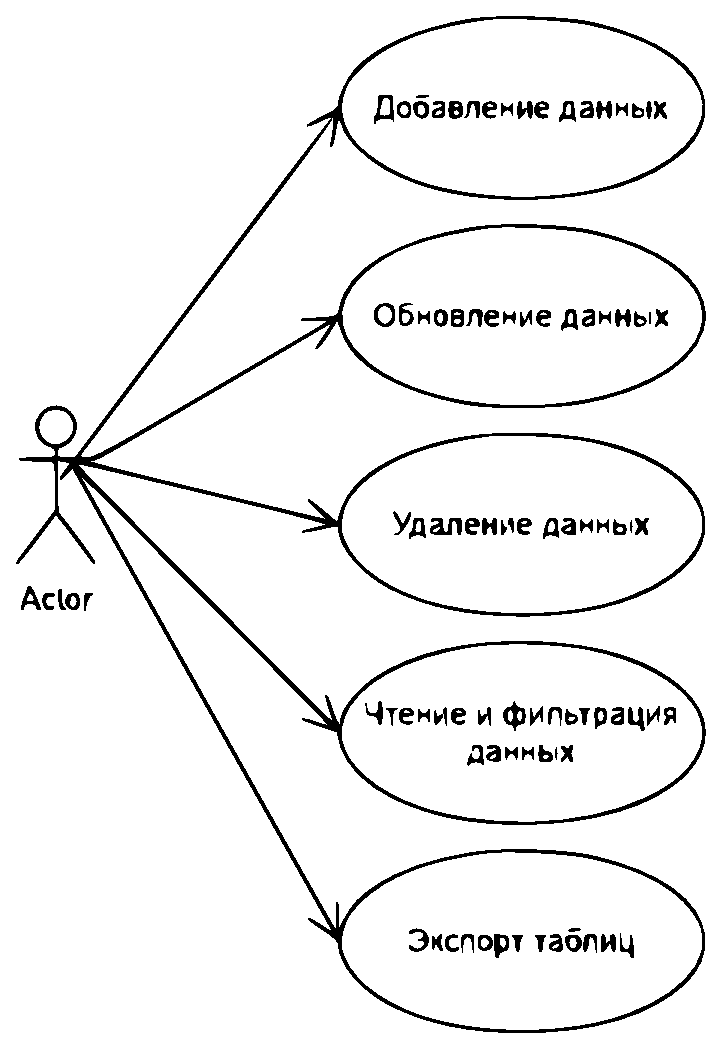
\includegraphics[width=1\linewidth]{prec}}
	\caption{Диаграмма прецедентов}
	\label{prec:image}
\end{figure}

\subsection{Требования к оформлению документации}

Разработка программной документации и программного изделия должна производиться согласно ГОСТ 19.102-77 и ГОСТ 34.601-90. Единая система программной документации.

\section{Технический проект}
\subsection{Общая характеристика организации решения задачи}

Необходимо спроектировать и разработать СУБД, которая должна способствовать хранению и фильтрации данных.

Система управления базами данных представляет собой набор взаимосвязных функций и макроссов, которые отвечают за работу с таблицами. БД представляет собой хэш-таблицу со структурами таблиц пользователей, которые имеют такие поля: название, списки колонок, списки столбцов.

\subsection{Обоснование выбора технологии проектирования}

На сегодняшний день информационный рынок, поставляющий программные решения в выбранной сфере, предлагает множество продуктов, позволяющих достигнуть поставленной цели – разработки СУБД.

\subsubsection{Описание используемых технологий и языков программирования}

В процессе разработки СУБД используются программные средства и языки программирования. Каждое программное средство и каждый язык программирования применяется для круга задач, при решении которых они необходимы.

\subsubsection{Язык программирования Lisp}

Lisp - это один из старейших языков программирования высокого уровня, созданный в 1958 году Джоном Маккарти. Первоначально он был разработан для исследований в области искусственного интеллекта и быстро стал одним из самых популярных языков для решения задач, связанных с обработкой данных, символическим вычислением и логическим выводом.

\paragraph{Основные особенности языка программирования Lisp}

\begin{enumerate} 
\item Символьная обработка. 
\item Простота синтаксиса.
\item Поддержка функционального программирования.
\item Макросы.
\item Множество диалектов.
\end{enumerate}

\subsection{Диаграмма компонентов и схема обмена данными между файлами компонента}

Диаграмма компонентов описывает особенности физического представления разрабатываемой системы. Она позволяет определить архитектуру системы, установив зависимости между программными компонентами, в роли которых может выступать как исходный, так и исполняемый код. Основными графическими элементами диаграммы компонентов являются компоненты, интерфейсы, а также зависимости между ними. На рисунке \ref{comp:image} изображена диаграмма компонентов для проектируемой системы. 

\begin{figure}[ht]
\center{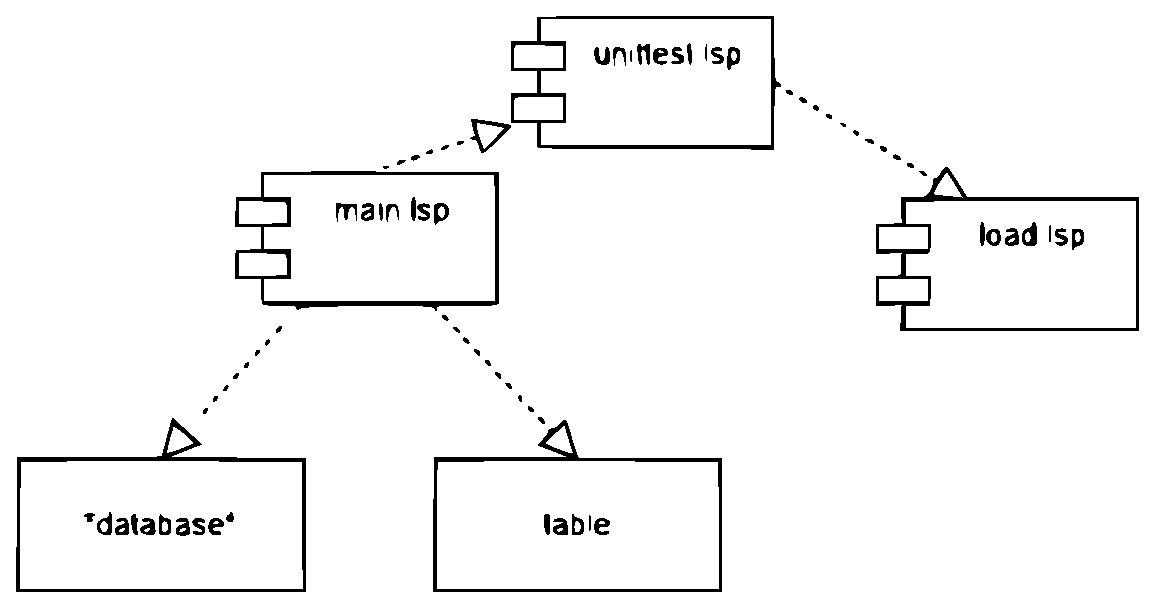
\includegraphics[width=1\linewidth]{comp}}
\caption{Диаграмма компонентов}
\label{comp:image}
\end{figure}

\ifПрактика{}\else{
   \section{Рабочий проект}
\subsection{Структуры, используемые при разработке СУБД}

Можно выделить следующий список структур и их методов, использованных при разработке СУБД (таблица \ref{class:table}).

\renewcommand{\arraystretch}{0.8} % уменьшение расстояний до сетки таблицы
\begin{xltabular}{\textwidth}{|X|p{2.5cm}|>{\setlength{\baselineskip}{0.7\baselineskip}}p{4.85cm}|>{\setlength{\baselineskip}{0.7\baselineskip}}p{4.85cm}|}
\caption{Описание структур, используемых в СУБД\label{class:table}}\\
\hline \centrow \setlength{\baselineskip}{0.7\baselineskip} Название структуры & \centrow \setlength{\baselineskip}{0.7\baselineskip} Модуль, к которому относится структура & \centrow Описание структуры & \centrow Методы \\
\hline \centrow 1 & \centrow 2 & \centrow 3 & \centrow 4\\ \hline
\endfirsthead
\caption*{Продолжение таблицы \ref{class:table}}\\
\hline \centrow 1 & \centrow 2 & \centrow 3 & \centrow 4\\ \hline
\finishhead
table & main & table – основная структура приложения. Имеет такие поля как: name, rows, columns. & Нет.\\
\end{xltabular}
\renewcommand{\arraystretch}{1.0} % восстановление сетки

\subsection{Описание функций системы управления базами данных}

\begin{enumerate}
\item create-table -- функция для создания таблицы. 
\item insert-into -- функция для вставки данных в таблицу.
\item make-select-from -- макрос для выборки данных по различным критериям.
\item delete-from -- функция для удаления данных из таблицы.
\item drop-table -- функция для удаления таблицы.
\item backup-table -- функция для создании копии таблицы в другую таблицу.
\item save-table-to-file -- функция для записи таблицы в другой файл.
\item make-update -- макрос для обновления данных по различным критериям.
\end{enumerate}

\subsection{Автоматизированное тестирование СУБД}

Один из автоматизированных тестов функций СУБД представлен на рисунке \ref{unittest:image}.

\begin{figure}[ht]
\begin{lstlisting}[language=Lisp]
(defun test-select-from (table-name columns rows selected-columns expected-result &optional condition)
(create-table table-name columns)
(dolist (row rows)
(insert-into table-name row))
(let ((result (select-from table-name selected-columns condition)))
(as-eq "test-select-from" result expected-result)))
\end{lstlisting}  
\caption{Автоматизированный тест функции}
\label{unittest:image}
\end{figure}

Вызов теста может осуществляться с разными входными данными. Пример представлен на рисунке \ref{unittestEx:image}.

\begin{figure}[ht]
\begin{lstlisting}[language=Lisp]
		(test-select-from 'test-table1211
		'((id integer) (name string) (age integer))
		'(((id . 1) (name . "egor") (age . 19))
		((id . 2) (name . "admin") (age . 24))
		((id . 3) (name . "alex") (age . 26)))
		'(name)
		'(((name . "admin")))
		'((> age 23) (/= name "alex")))
\end{lstlisting}  
\caption{Вызов автоматизированного теста функции}
\label{unittestEx:image}
\end{figure}

   \section*{ЗАКЛЮЧЕНИЕ}
\addcontentsline{toc}{section}{ЗАКЛЮЧЕНИЕ}

В результате выполнения курсовой работы была разработана система управления базами данных на языке программирования Lisp, ориентированной на практическое применение в реальных условиях.
 
Основные результаты работы:

\begin{enumerate}
\item Проведен анализ предметной области.
\item Разработана концептуальная модель системы управления базами данных.  Определены требования к системе.
\item Осуществлено проектирование СУБД. Разработана архитектура взаимодействия СУБД с пользователем.
\item Реализована и протестирована СУБД. Проведено автоматизированное тестирование.
\end{enumerate}

Все требования, объявленные в техническом задании, были полностью реализованы, все задачи, поставленные в начале разработки проекта, были также решены.

Готовый рабочий проект представлен программным интерфейсом системы управления базы данных для интеграции в различные проекты.  

}\fi
\addcontentsline{toc}{section}{СПИСОК ИСПОЛЬЗОВАННЫХ ИСТОЧНИКОВ}

\begin{thebibliography}{9}

    \bibitem{lisp1} Сайбель Питер, С.П. Практическое использование Common Lisp / С.П. Сайбель Питер. – М. СПб. : Питер, 2017. – 615 с. – ISBN 978-5-97060-538-7. – Текст~: непосредственный.
    \bibitem{lisp2} Грэм Пол, Г. П. ANSI Common Lisp / Г. П. Грэм Пол. – Москва : Бомбора, 2017. – 498 с. – ISBN 978-5-93286-206-3.. – Текст~: непосредственный.
    \bibitem{sql1} Шилдс, Ш. У. SQL: быстрое погружение / Ш. У. Шилдс. – М. СПб. : Питер, 2022. – 254 с. – ISBN 978-5-4461-1835-9.. – Текст~: непосредственный.
    \bibitem{sql2}	Моргунов, Е. П. PostgreSQL. Основы языка SQL / Е. П. Моргунов. – Москва : БХВ, 2022. – 336 с. – ISBN 978-5-9775-4022-3. – Текст~: непосредственный.
	\bibitem{arch}	Роберт, М. Чистая архитектура. Искусство разработки программного обеспечения / М. Роберт. – М. СПб. : Питер, 2022. – 592 с. – ISBN 978-5-4461-0772-8. – Текст~: непосредственный.
	\bibitem{arch2}	Head First. Паттерны проектирования. 2-е издание / Эрик Фримен, Элизабет Робсон, Кэтти Сьерра, Берт Бейтс. – М. СПб. : Питер, 2021. – 640 с. – ISBN 978-5-4461-1819-9. – Текст~: непосредственный.
	\bibitem{arch3}	Бхаргава, Адитья Грокаем алгоритмы. Иллюстрированное пособие для программистов и любопытствующих / Адитья Бхаргава. – М. СПб. : Питер, 2022. – 288 с. – ISBN 9785446109234. – Текст~: непосредственный.
	\bibitem{sql4}	Бондарь, А.Г. Microsoft SQL Server 2022 / А.Г. Бондарь. – Москва : БХВ, 2022. – 528 с. – ISBN 978-5-9775-1805-5. – Текст~: непосредственный.
	\bibitem{func}	Фридман, Д.П. THE LITTLE SCHEMER: Чудесное функциональное программирование / Д.П. Фридман. – Москва : Наука и техника, 2024. – 230 с. – ISBN 978-5-93700-234-1. – Текст~: непосредственный.    
	\bibitem{site}	Metanit : сайт. – URL: https://metanit.com/sql/mysql/2.1.php (дата обращения: 11.01.2025)    
	\bibitem{site2}	GitHub : сайт. – URL: https://github.com/sqlalchemy/sqlalchemy (дата обращения: 11.01.2025)    
\end{thebibliography}

\ifВКР{\appendix{Представление графического материала}

Графический материал, выполненный на отдельных листах,
изображен на рисунках А.1--А.\arabic{числоПлакатов}.
\setcounter{числоПлакатов}{0}

\renewcommand{\thefigure}{А.\arabic{figure}} % шаблон номера для плакатов

\begin{landscape}

\begin{плакат}
    \includegraphics[width=0.82\linewidth]{плакат1.png}
    \заголовок{Сведения о ВКРБ}
    \label{pl1:image}      
\end{плакат}

\begin{плакат}
    \includegraphics[width=0.82\linewidth]{плакат2.png}
    \заголовок{Цель и задачи разработки}
    \label{pl2:image}      
\end{плакат}

\begin{плакат}
    \includegraphics[width=0.82\linewidth]{плакат3.png}
    \заголовок{Концептуальная модель сайта}
    \label{pl3:image}      
\end{плакат}

\begin{плакат}
    \includegraphics[width=0.82\linewidth]{плакат3.png}
    \заголовок{Еще плакат}
    \label{pl4:image}      
\end{плакат}

\end{landscape}
}\fi
\ifПрактика{}\else{\appendix{Фрагменты исходного кода программы}

main.lsp
\begin{lstlisting}[language=Lisp]
	(defpackage :DBMS-package
	(:use :cl))
	
	(defstruct table
	name
	rows
	columns)
	
	(defvar *database* (make-hash-table :test 'equal))
	
	; Функции для работы с таблицей
	(defun create-table (name &optional columns)
	(progn
	(unless (gethash name *database*)
	(setf (gethash name *database*) (make-table :name name :columns columns :rows nil)))
	1))
	
	(defun insert-into (table-name row-data)
	(let ((table (gethash table-name *database*)))
	(if table
	(let* ((columns (table-columns table))
	(column-names (get-column-names columns)))
	;;Проверка, что все переданные ключи есть в колонках таблицы, ключи приводятся из  строкового формата в знаковый
	(if (every (lambda (col) (member (intern (string-upcase (string col))) column-names :test 'eq)) (mapcar #'car row-data))
	(progn
	(push row-data (table-rows table)))
	;; (format t "Rows ~a inserted into~%" row-data))
	(format t "ERROR: Some columns is not exist in table ~a~%" table-name)))
	(format t "ERROR: Table ~a not found!~%" table-name))))
	
	(defun select-all (table-name)
	(let ((table (gethash table-name *database*)))
	(if table
	(table-rows table)
	(progn
	(format t "ERROR: Table ~a not found!~%")
	nil))))
	
	
	(defun delete-from (table-name cond-pair)
	(let ((table (gethash table-name *database*)))
	(if table
	(let ((new-rows (remove-if (lambda (row) (every (lambda (condit) (equal (cdr condit) (cdr (assoc (car condit) row)))) cond-pair)) (table-rows table))))
	(setf (table-rows table) new-rows)
	(format t "Rows matching ~a deleted from table ~a.~%" cond-pair table-name) new-rows)
	(format t "ERROR: Table ~a not found!~%" table-name))))
	
	(defun drop-table (table-name)
	(if (gethash table-name *database*)
	(progn
	(remhash table-name *database*)
	(format t "Table ~a dropped!~%" table-name)
	1)
	(progn
	(format t "ERROR: Table ~a not found!~%" table-name)
	nil)))
	
	(defun backup-table (table-name backup-name)
	(let ((table (gethash table-name *database*)))
	(if table
	(progn
	(setf (gethash backup-name *database*)
	(make-table    :name (table-name table)
	:columns (copy-list (table-columns table))
	:rows (copy-list (table-rows table))))
	(progn
	(format t "Backup of table ~a success, create backup table ~a!~%" table-name backup-name)
	1))
	(progn
	(format t "ERROR: Table ~a nor found!~%" table-name)
	nil))))
	
	(defun save-table-to-file (table-name file-path)
	(let ((table (gethash table-name *database*)))
	(if table
	(with-open-file (stream file-path :direction :output 
	:if-exists :supersede
	:if-does-not-exist :create)
	(let ((columns (table-columns table)))
	;; Запись заголовков
	(format stream "~{~A~^,~}~%" (mapcar #'car columns))
	;; Запись строк
	(dolist (row (table-rows table))
	(format stream "~{~A~^,~}~%" 
	(mapcar (lambda (col) (cdr (assoc (car col) row)))  columns))))
	1)
	(format t "ERROR: Table ~a not found!~%" table-name))))			 
	
	(defun table-exist (table-name)
	(not (null (gethash table-name *database*))))
	
	(defun get-column-names (columns)
	(mapcar (lambda (col) (intern (string (car col)))) columns))
	
	(defun filter (predicate rows)
	"Фильтрует строки rows, оставляя только те, которые удовлетворяют предикату predicate."
	(remove-if-not predicate rows))
	
	(defun gen-vars (table)
	(mapcar (lambda (col)
	`(,col (cdr (assoc ',col row))))
	(mapcar #'car (table-columns table))))
	
	(defmacro create-condition (conditions)
	`(lambda (row)
	(every (lambda (condition)
	(cond
	;; Условие вида (< age 30)
	((and (listp condition)
	(symbolp (car condition))
	(symbolp (cadr condition)))
	(let* ((col (cadr condition))
	(op (car condition))
	(val (caddr condition))
	(row-val (cdr (assoc col row))))
	(case op
	((=) (equal row-val val))
	((>) (> row-val val))
	((<) (< row-val val))
	((>=) (>= row-val val))
	((<=) (<= row-val val))
	((/=) (not (equal row-val val)))
	(otherwise (error "Unsupported operator: ~a~%" op)))))
	
	;; Условие вида (name . "Egor")
	((and (consp condition)
	(symbolp (car condition)))
	(let ((key (car condition))
	(value (cdr condition)))
	(equal value (cdr (assoc key row)))))
	
	((or (stringp condition) (not (consp condition)))
	(error "Unsupported condition format: ~a~%" condition))
	
	(t (error "Unsupported condition format: ~a~%" condition))))
	,conditions)))
	
	(defmacro make-select-from (table-name columns &body body)
	`(let ((table (gethash ,table-name *database*)))
	(if table
	(let ((table-columns (mapcar #'car (table-columns table))))
	;; Проверка наличия всех выбранных столбцов
	(if (every (lambda (col) 
	(member (intern (string-upcase (string col))) table-columns :test 'eq)) 
	,columns)
	(let* ((filtered-rows
	(remove-if-not (lambda (row) 
	(let () ;;,(gen-vars table) (id (cdr (assoc 'id row)))
	,@body)) ;; Выполняем действия полученные из body
	(table-rows table))))
	;; Вывод столбцов
	(mapcar (lambda (row) 
	(remove-if-not (lambda (pair) 
	(member (car pair) ,columns :test 'equal))
	row))
	filtered-rows))
	(progn
	(format t "ERROR: Columns ~a not found in table ~a.~%" ,columns ,table-name)
	nil)))
	(progn
	(format t "ERROR: Table ~a not found!~%" ,table-name)
	nil))))
	
	(defmacro make-update (table-name updates &body body)
	`(let* ((table (gethash ,table-name *database*))
	(rows (table-rows table)))
	(let ((updated-rows
	(mapcar
	(lambda (row)
	(let ,(mapcar (lambda (col)
	`(,col (cdr (assoc ',col row))))
	(mapcar #'car (table-columns table)))
	(if (progn ,@body) ; Выполняем условия
	(let ((new-row (copy-list row)))
	(dolist (update ',updates)
	(let ((col (car update))
	(val (cdr update)))
	(setf (cdr (assoc col new-row)) val)))
	new-row)
	row))) ; Если условие не выполнено, строка остаётся неизменной
	rows)))
	(setf (table-rows table) updated-rows)
	1)))
\end{lstlisting} 

unittest.lsp
\begin{lstlisting}[language=Lisp]
	(load "./main.lsp")
	(format t "Файл main.lsp загружен~%")
	;(in-package :DBMS-package)
	
	(defun test-create-table (table-name &optional columns expected-result)
	(let ((result (create-table table-name columns)))
	(as-eq "test-create-table" result expected-result)))
	
	(defun test-insert-into (table-name columns row expected-row)
	(create-table table-name columns)
	(insert-into table-name row)
	(let ((table (gethash table-name *database*)))
	(if table
	(let ((actual-row (first (table-rows table))))
	(as-eq "test-insert-into" actual-row expected-row))
	(format t "ERROR: Table ~a не найдена в базе данных~%" table-name))))
	
	(defun test-select-from (table-name columns rows selected-columns expected-result &optional condition)
	(create-table table-name columns)
	(dolist (row rows)
	(insert-into table-name row))
	(let ((result (select-from table-name selected-columns condition)))
	(as-eq "test-select-from" result expected-result)))
	
	(defun test-select-all (table-name columns rows expected-result)
	(create-table table-name columns)
	(dolist (row rows)
	(insert-into table-name row))
	(let ((result (select-all table-name)))
	(as-eq "test-select-all" result expected-result)))
	
	(defun test-drop-table (table-name columns expected-result)
	(create-table table-name columns)
	(let ((result (drop-table table-name)))
	(as-eq "test-drop-table" result expected-result)))
	
	(defun test-update-data (table-name columns rows id field-name new-value expected-result)
	(create-table table-name columns)
	(dolist (row rows)
	(insert-into table-name row))
	(let ((result (update table-name id field-name new-value))) 
	(as-eq "test-update" result expected-result)))
	
	(defun test-backup-table (table-name columns rows backup-name expected-result)
	(create-table table-name columns)
	(dolist (row rows)
	(insert-into table-name row))
	(let ((result (backup-table table-name backup-name)))
	(as-eq "test-backup-table" result expected-result)))
	
	(defun test-save-table-to-file (table-name columns rows path expected-result)
	(create-table table-name columns)
	(dolist (row rows)
	(insert-into table-name row))
	(let ((result (save-table-to-file table-name path)))
	(as-eq "test-save-table-to-file" result expected-result)))
	
	(defun test-create-condition ()
	(let* ((rows '(((id . 1) (name . "Alice") (age . 25))
	((id . 2) (name . "Egor") (age . 30))
	((id . 3) (name . "Alex") (age . 35))))
	;; Условие: возраст < 30
	(condition1 (create-condition '((< age 30))))
	;; Условие: возраст между 20 и 40
	(condition3 (create-condition '((>= age 30) (/= name "Alex")))))
	(format t "Rows matching condition1: ~a~%" (remove-if-not condition1 rows))
	(format t "Rows matching condition3: ~a~%" (remove-if-not condition3 rows))))
	
	(defun mk-sel-from ()
	(create-table 'tab1 '((id integer) (name string) (age integer)))  
	(insert-into 'tab1 '((id . 1) (name . "alex") (age . 25)))     
	(insert-into 'tab1 '((id . 2) (name . "egor") (age . 54)))
	(insert-into 'tab1 '((id . 3) (name . "vova") (age . 14)))
	(insert-into 'tab1 '((id . 4) (name . "daniil") (age . 18)))
	(insert-into 'tab1 '((id . 5) (name . "alex") (age . 27)))
	
	(let ((result (make-select-from 'tab1 '(name age)
	(and (string= (cdr (assoc 'name row)) "alex")
	(> (cdr (assoc 'age row)) 20)))))
	(format t "Result make-select-from: ~a~%" result)))
	
	(defun mk-update-test ()
	(create-table 'tab1 '((id integer) (name string) (age integer)))
	(insert-into 'tab1 '((id . 1) (name . "alex") (age . 25)))     
	(insert-into 'tab1 '((id . 2) (name . "egor") (age . 54)))
	(insert-into 'tab1 '((id . 3) (name . "vova") (age . 14)))
	(insert-into 'tab1 '((id . 4) (name . "daniil") (age . 18)))
	(insert-into 'tab1 '((id . 5) (name . "alex") (age . 27)))
	
	(make-update 'tab1 '((age . 20)) (< (cdr (assoc 'age row)) 20))
	(let ((result (make-select-from 'tab1 '(id name age))))
	(format t "Result make-update: ~a~%" result)))
	
	
	(defun as-eq (test-name result expected)
	(if (equal result expected)
	(format t "~a: PASSED~%" test-name)
	(format t "~a: FAILED - ожидалось ~a, но было полученно ~a~%" test-name expected result)))
	
	(defun run-unittest ()
	(format t "Начало тестирования...~%~%")
	(test-gen-vars)
	(test-create-condition)
	;; Тестирование создания таблицы.
	(test-create-table 'test-table01 '((id . 1) (name . "adm")) 1)
	;; Тестирование вставки данных в таблицу.
	(test-insert-into 'users '((id integer) (name string) (age integer))
	'((id . 1) (name . "adm") (age . 24))
	'((id . 1) (name . "adm") (age . 24)))
	(test-drop-table 'test-table111 '((id integer) (name string) (age integer)) 1)
	;; Тестирование чтения данных из таблицы без условия.
	(test-select-from 'test-table111
	'((id integer) (name string) (age integer))
	'(((id . 1) (name . "egor") (age . 19))
	((id . 2) (name . "admin") (age . 24)))
	'(name)
	'(((name . "admin")) ((name . "egor")))
	nil)
	;; Тестирование чтения данных из таблицы с условием.
	(test-drop-table 'test-table1211 '((id integer) (name string)) 1)
	(test-select-from 'test-table1211
	'((id integer) (name string) (age integer))
	'(((id . 1) (name . "egor") (age . 19))
	((id . 2) (name . "admin") (age . 24))
	((id . 3) (name . "alex") (age . 26)))
	'(name)
	'(((name . "admin")))
	'((> age 23) (/= name "alex")))
	;; Тестирование удаления таблицы.
	(test-drop-table 'table1 '((id integer) (name string)) 1)
	;; Тестирование чтения всех данных из таблицы.
	(test-select-all 'table1 '((id integer) (name string))
	'(((id . 1) (name . "adm"))
	((id . 2) (name . "adm1")))
	'(((id . 2) (name . "adm1"))
	((id . 1) (name . "adm"))))
	;; Тестирование функции обновления данных по id
	(test-drop-table 'table999 '((id integer) (name string) (age integer)) 1)
	(test-update-data 'table999 '((id integer) (name string) (age integer))
	'(((id . 1) (name . "egor") (age . 19))
	((id . 2) (name . "admin") (age . 24)))
	1
	'name
	"update-egor"
	'((id . 1) (name . "update-egor") (age . 19)))
	;; Тестирование функции создания копии таблицы
	(test-backup-table 'table2213 '((id integer) (name string) (age integer))
	'(((id . 1) (name . "egor"))
	((id . 2) (name . "alex"))
	((id . 3) (name . "asd")))
	'backup-table2213
	1)
	;; Тестирование функции записи таблицы в CSV файл
	(test-drop-table 'table2214 '((id integer) (name string) (age integer)) 1)
	(test-save-table-to-file 'table2214 '((id integer) (name string) (age integer))
	'(((id . 1) (name . "alex") (age . 23))
	((id . 2) (name . "egor") (age . 24))
	((id . 3) (name . "vova") (age . 25))
	((id . 4) (name . "daniil") (age . 12)))
	"output.txt"
	1)
	(test-drop-table 'tab1 '((id integer) (name string) (age integer)) 1)
	(mk-sel-from)
	(test-drop-table 'tab1 '((id integer) (name string) (age integer)) 1)
	(mk-update-test)
	
	(format t "~%Тестирования завершенно.~%"))
\end{lstlisting}  

\ifВКР{
\newpage
\addcontentsline{toc}{section}{На отдельных листах (CD-RW в прикрепленном конверте)}
\begin{center}
\textbf{Место для диска}
\end{center}
}\fi
}\fi
\end{document}
